Given the ethical and societal implications of algorithm-driven
decisions, understanding the underlying methodologies is essential.
Among these, hierarchical clustering stands out as an influential
unsupervised learning technique widely applied to discover natural
groupings and reveal intrinsic structures within complex data. Its
flexibility in cases where the number of clusters is unknown
beforehand makes it particularly valuable, adapting to various
analytical contexts.

\subsection{Structure and Representation}\label{subsec:hierarchical_clustering}

Hierarchical clustering organizes a dataset \(X\) into a structured
hierarchy of nested clusters, represented by a tree-like diagram
known as a \textit{dendrogram}. Each leaf node corresponds to an
individual data point, while internal nodes represent clusters formed
through either merging or splitting of points. The dendrogram offers
a multi-resolution view, enabling users to explore and select
clusters at varying degrees of granularity. Unlike flat clustering
methods (e.g., \(k\)-means), hierarchical methods do not require
pre-specification of the number of clusters, providing a flexible
structure adaptable to different analytical needs.

\begin{figure}[h]
  \centering
  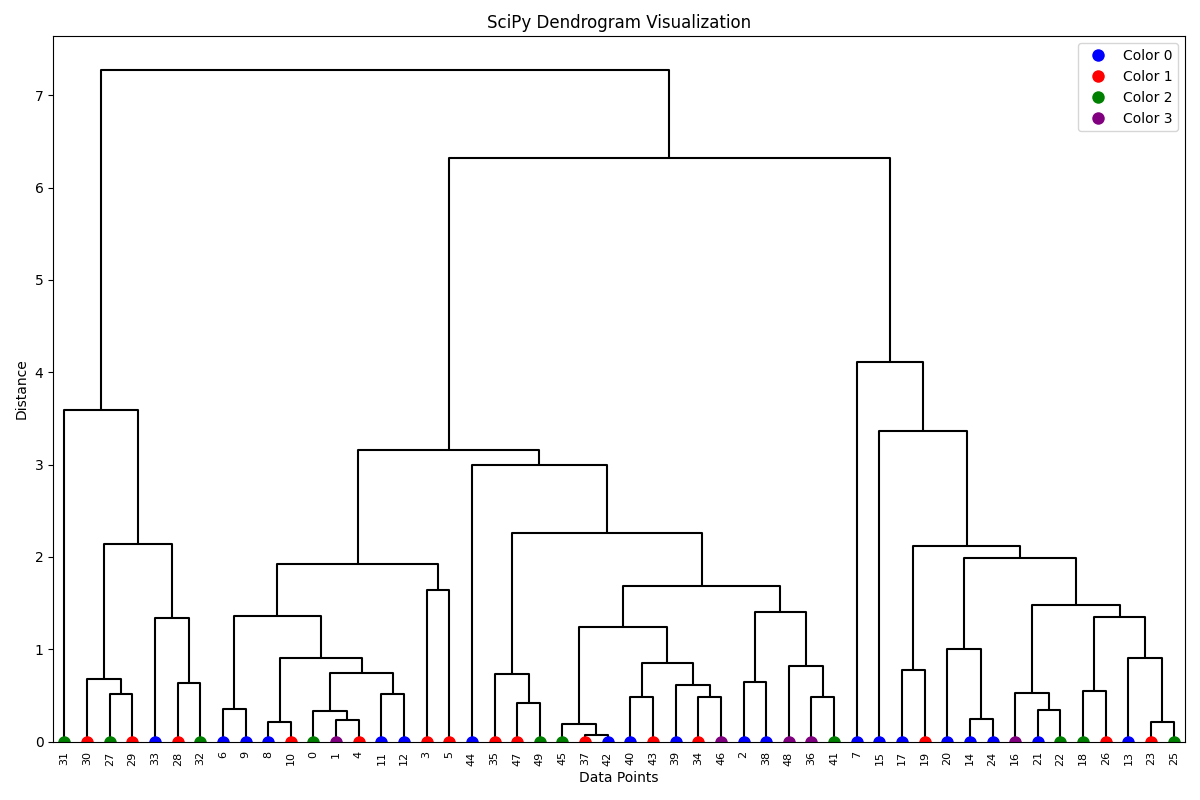
\includegraphics[width=0.9\textwidth]{sections/background/scipy_dendrogram.png}
  \caption{An example of a dendogram representation.}
  \label{fig:example-dendogram}
\end{figure}

Formally, hierarchical clustering constructs a nested partitioning of
a dataset \(X\), such that each cluster at a given resolution is
entirely contained within clusters at coarser resolutions, ensuring
consistency across hierarchical levels.

Hierarchical clustering methods are broadly categorized into two
complementary approaches: \textit{agglomerative} (bottom-up) and
\textit{divisive} (top-down).

\paragraph{Agglomerative Clustering (Bottom-Up Approach).}
Agglomerative hierarchical clustering (AHC) begins with each data
point as a singleton cluster. Clusters are iteratively merged
according to their proximity, defined by a linkage criterion, until
all points form a single cluster. The choice of linkage significantly
impacts the structure and characteristics of resulting clusters.
Some common linkage methods are listed below, however, these are
numerous and the choice of linkage criterion is highly dependent on
the application and underlying data. [SCIPY DOCS HAVE CITS]

\begin{itemize}
  \item \textbf{Single-Linkage:} This method defines the distance
    between two clusters by the shortest distance between any point
    in one cluster and any point in the other. It is known to capture
    irregular cluster shapes but can suffer from a “chaining effect,”
    where clusters may form long, snake-like structures.
    \begin{align*}
      \min_{a \in A, b \in B} d(a, b)
    \end{align*}

  \item \textbf{Complete-Linkage:} This method measures the distance
    between two clusters by looking at the maximum distance between
    any point in one cluster and any point in the other. It typically
    yields compact, roughly spherical clusters, and is robust against
    outliers because it considers the farthest pair of points.
    \begin{align*}
      \max_{a \in A, b \in B} d(a, b)
    \end{align*}

  \item \textbf{Average-Linkage (UPGMA):} In this approach, the
    distance between two clusters is computed as the average distance
    between all pairs of points (one from each cluster). This often
    produces balanced clusters and has widespread empirical success
    across diverse applications.
    \begin{align*}
      \frac{1}{|A| \cdot |B|} \sum_{a \in A} \sum_{b \in B} d(a, b)
    \end{align*}

  \item \textbf{Centroid-Linkage:} This method uses the distance
    between the centroids (mean positions) of two clusters. It forms
    clusters that tend to be spherical, and it has comparatively
    moderate computational requirements.
    \begin{align*}
      \| \mu_A - \mu_B \|^2
      \quad \text{(where $\mu_A$ and $\mu_B$ are centroids of A and B)}
    \end{align*}

  \item \textbf{Ward’s Method:} This approach merges the pair of
    clusters that leads to the smallest increase in the overall
    within-cluster variance (sum of squared distances) at each step.
    Although its mathematical formulation can be quite involved (and
    hence is omitted here), the end result is the creation of cohesive,
    balanced clusters. However, it can be more computationally
    expensive for large datasets.
\end{itemize}

The agglomerative approach's primary advantage lies in its conceptual
simplicity, interpretability, and deterministic nature, but it
typically incurs a computational complexity of \(O(n^2\log n)\) or
\(O(n^3)\), depending on the linkage method and implementation.

\paragraph{Divisive Clustering (Top-Down Approach).}
Divisive hierarchical clustering operates in the reverse direction:
it begins by placing all data points into a single comprehensive
cluster. At each iteration, this cluster is recursively split into
smaller clusters according to a specified criterion—often focusing on
maximizing inter-cluster distance or minimizing intra-cluster
similarity—until each cluster contains only one data point.

Divisive clustering provides a complementary perspective to
agglomerative methods, allowing potentially clearer initial
partitioning of the data. However, divisive algorithms generally
require greater computational resources, as optimal splitting is
typically more computationally intensive than merging clusters. Due
to this increased complexity, divisive clustering is less commonly
used in practice but is valuable in contexts where meaningful
top-level partitions are prioritized.

\subsection{Cost Functions in Hierarchical Clustering}
To quantitatively assess and optimize hierarchical clustering,
researchers have proposed explicit \textbf{cost functions}
\cite{dasgupta2016cost}. These functions take an input graph and a
hierarchical clustering (represented by a tree) and output a value
representing the goodness of the hierarchy.

\paragraph{Dasgupta's cost function} is a formal,
pairwise-similarity-based objective that allows rigorous evaluation
and comparison of hierarchical clustering outcomes
\cite{dasgupta2016cost}. Given a weighted similarity graph
$G=(V,E,w)$, the cost of a hierarchy $T$ is defined as:

\begin{equation*}
  \text{cost}_G(T) = \sum_{e=(x,y) \in E} w(e) \cdot |T_{xy}|
\end{equation*}

where $|T_{xy}|$ is the size of the smallest cluster in $T$
containing both $x$ and $y$. A higher cost indicates that similar
points are clustered loosely in the hierarchy, which is undesirable.
Optimizing Dasgupta's cost function is NP-hard, and the best known
approximation algorithm has a factor of $O(\sqrt{\log n})$.

\paragraph{Mosley's Revenue}
proposed by Moseley and Wang, is defined in the
context of similarity edge weights. It is closely related to cost,
but instead of multiplying the edge weight by the size of the
smallest containing cluster, it uses a related measure. Revenue and
cost are dual to each other, meaning a hierarchy optimizing one also
optimizes the other. Average linkage is a constant-factor
approximation for revenue.

\paragraph{Cohen's Value}
introduced by Cohen-Addad et al.
[\cite{cohen}], is defined in the context where edge
weights represent differences or dissimilarities. The formula for
value is the same as for cost, but because the context of edge
weights is different, it becomes a maximization function. Similar to
revenue, average linkage is a constant-factor approximation for value.

\paragraph{}These cost functions allow for theoretical evaluation of
hierarchical clustering algorithms.

\subsection{Applications of Hierarchical Clustering.}
Hierarchical clustering's flexibility and interpretability have
enabled it to become pervasive across diverse application areas.
Notable examples include:

\paragraph{Computational Biology and Bioinformatics:} Widely
employed for gene expression analysis to discover clusters of
co-expressed genes, thereby elucidating biological pathways and
functions. Additionally, hierarchical clustering underpins the
construction of phylogenetic trees, revealing evolutionary
relationships among species or genetic sequences.

\paragraph{Image Processing and Computer Vision:} Hierarchical
methods are integral to multi-scale image segmentation,
effectively organizing pixels into coherent regions at various
resolutions. Such techniques facilitate detailed scene
understanding, object detection, and content-based image retrieval.

\paragraph{Natural Language Processing (NLP):} Extensively
applied in document clustering to identify thematic groupings,
thereby enabling structured information retrieval, summarization,
and exploration of large textual corpora. Hierarchical clustering
is also instrumental in developing taxonomies and concept
hierarchies in ontology construction.

\paragraph{Marketing and Customer Analytics:} Businesses
frequently utilize hierarchical clustering for market
segmentation and customer profiling, revealing detailed consumer
segments based on purchasing behaviors, demographic attributes,
or online activities. This segmentation allows targeted marketing
and personalized recommendations.

\paragraph{Social Network Analysis:} Hierarchical clustering
aids in detecting community structures within networks, capturing
meaningful groupings such as social circles, influencer
communities, or collaborative groups. These structures can inform
targeted interventions, marketing strategies, or community
detection in online platforms.

\paragraph{Psychology and Sociology:} Researchers leverage
hierarchical clustering for psychometric data analysis and social
behavior pattern identification, uncovering latent constructs and
behavioral archetypes within populations. This facilitates
targeted policy-making, interventions, and sociocultural studies.

\paragraph{Healthcare and Medical Diagnostics:} Hierarchical
methods help classify patients based on symptom profiles or
diagnostic test results, improving patient stratification,
treatment personalization, and clinical decision support systems.

The broad applicability across these domains underscores hierarchical
clustering’s effectiveness in capturing complex structures inherent
to diverse datasets, aligning closely with many practical, societal,
and ethical contexts discussed earlier. Nonetheless, the
computational complexity of hierarchical clustering poses a
persistent challenge, especially with massive datasets.

Given hierarchical clustering’s use in sensitive domains like
healthcare, employment, and criminal justice, ensuring fairness
becomes ethically and practically critical. Integrating explicit
fairness constraints into hierarchical clustering—termed \textit{fair
hierarchical clustering} (FHC)—is thus essential to avoid
perpetuating existing biases.